\documentclass[12pt]{article}
\usepackage[margin=1in]{geometry}
\usepackage{setspace}
\onehalfspacing

% Start of preamble
%==========================================================================================%
% Required to support mathematical unicode
\usepackage[warnunknown, fasterrors, mathletters]{ucs}
\usepackage[utf8x]{inputenc}

\usepackage[dvipsnames,table,xcdraw]{xcolor}
\usepackage{hyperref} 
\hypersetup{
colorlinks=true,
linkcolor=blue,
filecolor=magenta,
urlcolor=cyan,
pdfpagemode=FullScreen
}

% Standard mathematical typesetting packages
\usepackage{amsmath,amssymb,amscd,amsthm,amsxtra, pxfonts}
\usepackage{mathtools,mathrsfs,dsfont,xparse}

% Symbol and utility packages
\usepackage{cancel, textcomp}
\usepackage[mathscr]{euscript}
\usepackage[nointegrals]{wasysym}
\usepackage{apacite}

% Extras
\usepackage{physics}  
\usepackage{tikz-cd}
\usepackage{quiver}
\usepackage{microtype}
\usepackage{enumitem}
\usepackage{titling}
\usepackage{graphicx}

% Fancy theorems due to @intuitively on discord
\usepackage{mdframed}
\newmdtheoremenv[
backgroundcolor=NavyBlue!30,
linewidth=2pt,
linecolor=NavyBlue,
topline=false,
bottomline=false,
rightline=false,
innertopmargin=10pt,
innerbottommargin=10pt,
innerrightmargin=10pt,
innerleftmargin=10pt,
skipabove=\baselineskip,
skipbelow=\baselineskip
]{mytheorem}{Theorem}

\newenvironment{theorem}{\begin{mytheorem}}{\end{mytheorem}}

\newtheorem{corollary}{Corollary}
\newtheorem{lemma}{Lemma}

\newtheoremstyle{definitionstyle}
{\topsep}%
{\topsep}%
{}%
{}%
{\bfseries}%
{.}%
{.5em}%
{}%
\theoremstyle{definitionstyle}
\newmdtheoremenv[
backgroundcolor=Violet!30,
linewidth=2pt,
linecolor=Violet,
topline=false,
bottomline=false,
rightline=false,
innertopmargin=10pt,
innerbottommargin=10pt,
innerrightmargin=10pt,
innerleftmargin=10pt,
skipabove=\baselineskip,
skipbelow=\baselineskip,
]{mydef}{Definition}
\newenvironment{definition}{\begin{mydef}}{\end{mydef}}

\newtheorem*{remark}{Remark}

\newtheorem*{example}{Example}

% Common shortcuts
\def\mbb#1{\mathbb{#1}}
\def\mfk#1{\mathfrak{#1}}

\def\bN{\mbb{N}}
\def \C{\mbb{C}}
\def \R{\mbb{R}}
\def\bQ{\mbb{Q}}
\def\bZ{\mbb{Z}}
\def \cph{\varphi}
\renewcommand{\th}{\theta}
\def \ve{\varepsilon}
\newcommand{\mg}[1]{\| #1 \|}

% Often helpful macros
\newcommand{\floor}[1]{\left\lfloor#1\right\rfloor}
\newcommand{\ceil}[1]{\left\lceil#1\right\rceil}
\renewcommand{\qed}{\hfill\qedsymbol}
\renewcommand{\P}{\mathbb P\qty}
\newcommand{\E}{\mathbb{E}\qty}
\newcommand{\Cov}{\mathrm{Cov}\qty}
\newcommand{\Var}{\mathrm{Var}\qty}

% Sets
\usepackage{braket}

\graphicspath{{/}}
\usepackage{float}

\newcommand{\SET}[1]{\Set{\mskip-\medmuskip #1 \mskip-\medmuskip}}

% End of preamble
%==========================================================================================%

% Start of commands specific to this file
%==========================================================================================%

%==========================================================================================%
% End of commands specific to this file

\title{CSE 421 HW4}
\date{\today}
\author{Rohan Mukherjee}

\begin{document}
    \maketitle

    \subsection*{Problem 1.}
    We give the following counter-example:
    \begin{figure}[H]
        \centering
        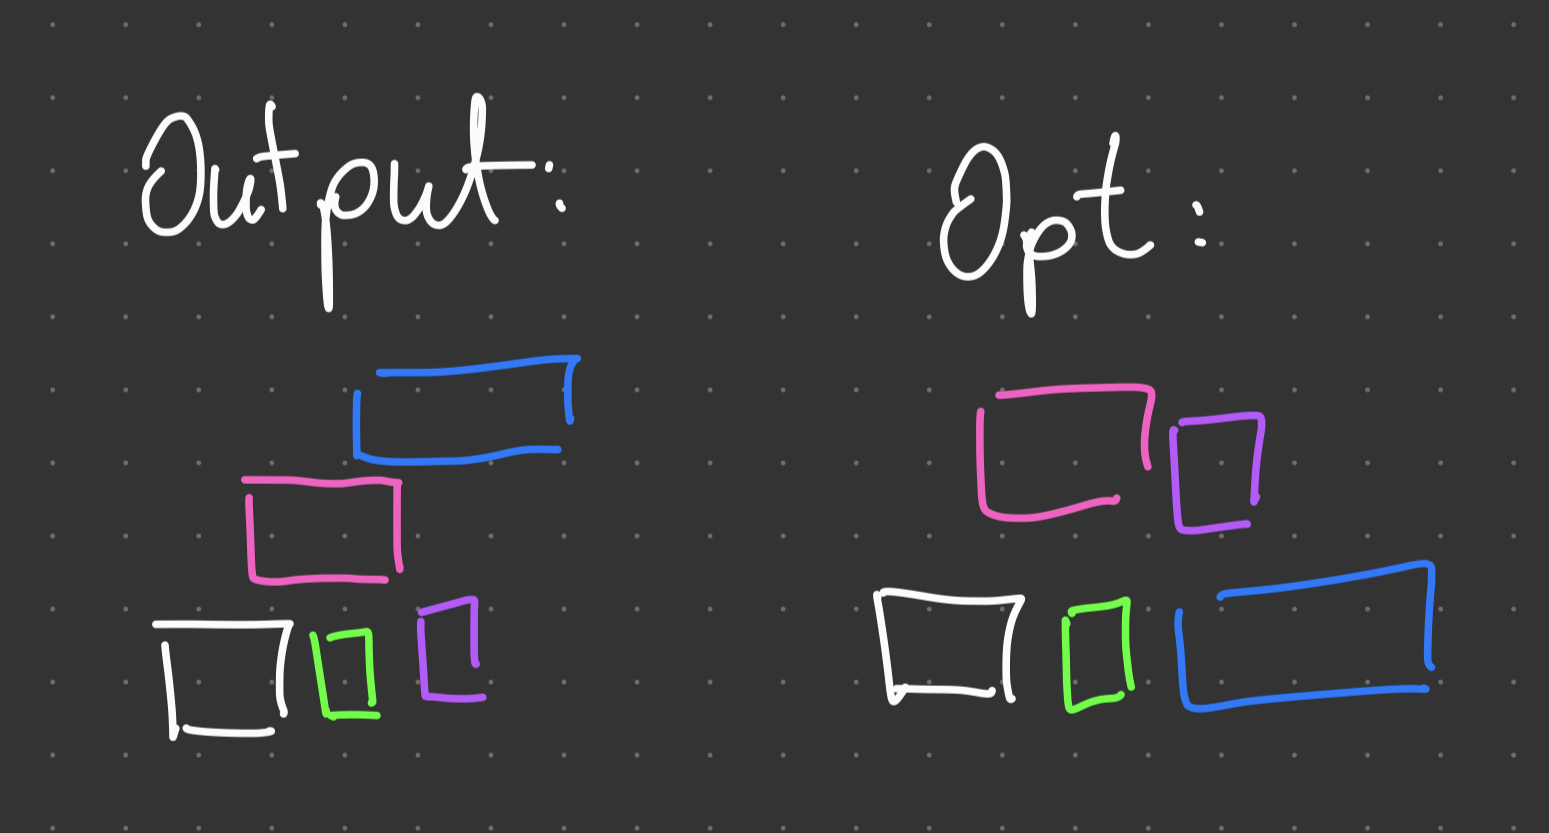
\includegraphics[width=0.8\textwidth]{counter.jpg}
        \caption{Greedy Output (Left) and Optimal Output (Right)}
    \end{figure}
    When we order the intervals by their finishing time, we get white, green, pink, purple, and finally blue. The greedy algorithm will first pick white, then it will add green to white's classroom since there is no overlap. Then it will see that pink has overlap, so it makes a new classroom for it. Then it moves onto purple, notices that it has no overlap with the first classroom, and adds it accordingly. Then it notices that blue overlaps with purple in the first classroom and pink in the second, and makes a third classroom for it. However, by putting the classes in the optimal configuration as shown on the right, we can see that our greedy algorithm is not optimal.

    \subsection*{Problem 2.}
    First, sort the numbers as $a_1, \ldots, a_n$. Then pair $a_n$ with $a_1$, $a_{n-1}$ with $a_2$, and so on, until you pair $a_{n/2+1}$ with $a_{n/2}$. The sorting takes $O(n \log n)$ time and the pairing takes $O(n)$ time, so this greedy algorithm runs in $O(n\log n)$ time, with the largest number paired with the smallest, second largest with the second smallest, and so on. Let \textbf{OPT} be the optimal solution. Suppose that \textbf{OPT} $\neq$ \textbf{GREEDY}. If the largest number $a_n$ in \textbf{OPT} is not paired with the smallest number $a_1$, let the pair of $a_n$ in \textbf{OPT} be $\SET{a_n, a_1+x}$ and the pair of the smallest be $\SET{a_1, a_n-y}$ for some $x,y \geq 0$. We seek to replace these pairs with $\SET{a_n, a_1}$ and $\SET{a_1+x, a_n-y}$. Notice that the sum of the second pair is $a_1+a_n+x-y \leq a_n+a_1+x$ which was sum of the original pair $\SET{a_n, a_1+x}$. Clearly the pair $\SET{a_1, a_n-y}$ is not larger than $\SET{a_n, a_1+x}$. So, if $\SET{a_n, a_1+x}$ was the largest pair, we have replaced it and precisely one other pair with values $a_1+a_n$, $a_1+a_n+x-y$ which are both $\leq a_n+a_1+x$. If $x > 0$, \textbf{OPT} is not optimal, a contradiction, otherwise we continue by moving the second largest and second smallest together, and so on until either \textbf{GREEDY} = \textbf{OPT} or we reach a contradiction.

    \subsection*{Problem 3.}
    Recall that if you add a non-tree edge to a minimum spanning tree you get one unique cycle. So, given a fixed edge $e \in T_1$, we can find a cycle $C$ containing $e$ in $T_2 + e$. We also know that $T_1 - e$ consists of precisely 2 connected components. Call these vertex sets $(S, \overline S)$. By what we proved in class, the cycle $C$ in $T_2 + e$ be cut at least twice (since $e$ is in the cut), so call the other edge $f$. We claim that $T_2 + e - f$ and $T_1 - f + e$ are both spanning trees. Since they both have $n-1$ edges (because the edge sets are disjoint), we just have to show they are connected. 
    
    Firstly, $T_1-e+f$ is clearly connected, since $(S, \overline S)$ were $T_1 - e$'s two connected components, and by construction $f$ crosses this cut and henceforth connects the two components. Since $T_2$ is connected, we know that every vertex $v \in T_2$ has a path to a vertex $w$ in the cycle. We can find a path using only non-cycle edges by simply truncating the path at the earliest point where it intersects the cycle. The only way this would result in an empty path is if $v$ was already in the cycle, which it was assumed not to be. Clearly, removing one edge $f$ from a cycle will still result in every vertex in the cycle being connected to each other. Thus we can find a path from any vertex $v$ to $w$ in $T_2$ by combining a path from $v$ to the cycle, the path from $w$ to the cycle, and the cycle's path from one of it's vertices to another (which are possibly the same). Thus $T_2 + e - f$ is connected, which completes the proof.
    \begin{figure}[H]
        \centering
        \begin{tikzcd}
            && 1 \\
            & 2 && 3 \\
            4
            \arrow[color={rgb,255:red,92;green,92;blue,214}, no head, from=1-3, to=2-2]
            \arrow[color={rgb,255:red,92;green,92;blue,214}, no head, from=1-3, to=2-4]
            \arrow[color={rgb,255:red,92;green,92;blue,214}, no head, from=2-2, to=3-1]
            \arrow[color={rgb,255:red,214;green,92;blue,92}, no head, from=2-4, to=2-2]
            \arrow[color={rgb,255:red,214;green,92;blue,92}, curve={height=-30pt}, no head, from=3-1, to=1-3]
            \arrow[color={rgb,255:red,214;green,92;blue,92}, no head, from=3-1, to=2-4]
        \end{tikzcd}
        \caption{Two Disjoint Edge Set Spanning Trees}
    \end{figure}
    In the above graph, if $e = (2,3)$ the cycle would be $\SET{1, 2, 3}$ and the edge $f$ would be $(1, 2)$.

    \subsection*{Problem 4.} 
    \begin{enumerate}[label=\alph*)]
        \item This translates to $T(n) = 7T(n/2) + O(n)$. Since $7 > 2^1$, we get 
        \begin{align*}
            T(n) = O(n^{\log_7(2)})
        \end{align*}
        
        \item This translates to $T(n) = 25T(n/5) + O(n^2)$. Since $25 = 5^2$ we get $T(n) = O(n^2\log n)$.
        \item This translates to $T(n) = 4T(n-4) + O(n)$. This gives $T(n) = O(4^{n/4})$ by the tree method.
    \end{enumerate}

    \subsection*{Problem 5.}
    Given the array input $n$, initialize an empty array called "left" of size $\floor{(n-1)/2}$, and "right" of size $\floor{n/2}$. Let $c = a_{\floor{n/2}}$. Replace the interval $[\ell, u]$ with the interval $[\ell-c, u-c]$. Let "count" be the number of interval sums that are in the right range. 
    
    Progressively fill up the "right" array by adding $a_{\floor{n/2}+1}, a_{\floor{n/2}+2}, \ldots$, checking at each step if the interval is in the range and adding to "count" accordingly, until we have seen every interval sum containing $c$ with $c$ as the smallest index. This obviously takes $O(n)$ time. Sort the right array (which takes $O(n\log n)$ time). 
    
    Now, add the first element on the left of $c$ to the current index sum, and if it is in the right range increse count accordingly. Call the sum of the elements currently in the index sum to the left of $c$ $T$. Replace the interval with $[\ell-c-T, u-c-T]$. Define a $\leq$ binary search algorithm as one that does a binary search, but if the value is not found return the value that is the closest and $\leq$ to the searched value, and similarly define a $\geq$ binary search. These can both be implemented in $O(1)$ time by running a normal binary search and checking the two adjacent elements for the one that is above and below the target for $\geq$ and $\leq$ respectively, and outputting $-1$ if neither are. Thus, both run in $O(\log n)$ time.
    
    Do a $\geq$ binary search on the value $\ell-c-T$ in the array "right" and similarly a $\leq$ binary search on the value $u-c-T$ on "right", which takes $O(\log n)$ time. If the value returned by the $\geq$ binary search or the value returned by the $\leq$ binary search on $u-c-T$ is $-1$ stop. Otherwise, we know that the intervals between these search results will be a complete list of the right interval sums that are in that range. Thus by taking the difference of their indices and adding 1, we get the number of right intervals in that range (taking $O(1)$ time). This gives a complete list of the right intervals that, when added to the current left interval, will be in the range. This procedure clearly then counts the number of intervals with smallest index the index of $c$ that are in the range, similarly the number of intervals with largest index equal to the index of $c$, and finally the number of intervals contianing $c$ in the interval, by construction. Thus we have found all the intervals containing $c$ in the interval. 
    
    Recursively call the algorithm on the numbers $a_1, \ldots, a_{\floor{(n-1)/2}}$ and $a_{\floor{n/2} + 1}, \ldots, a_n$. Notice since we have counted all the intervals containing $c$, we only need to count the intervals that are either to the left of $c$ or to the right. Clearly, if $n = 1$ then the algorithm already counts the number of intervals containing $a_1$ in the range as every interval contains $a_1$. Inductively assume the algorithm is correct for $\leq n-1$ elements. Since we call the algorithm on two arrays of size $\leq n/2$, by induction these count precisely the number of intervals to the left and right of $c$ in the range (resp.), so the algoirthm is correct.
    
    By summing up the above terms, we find the running time to be:
    \begin{align*}
        T(n) = 2T(n/2) + O(n\log n)
    \end{align*}
    The corresponding tree is:
    \[\begin{tikzcd}
        && {n\log n} &&& {n\log n} \\
        & {\frac{n}{2}\log(n/2)} && {\frac{n}{2}\log(n/2)} && {\leq n\log n} \\
        {\frac{n}4\log(n/4)} & {\frac{n}4\log(n/4)} && {\frac{n}4\log(n/4)} & {\frac{n}4\log(n/4)} & {\leq n\log n} \\
        \vdots & \vdots && \vdots & \vdots
        \arrow[from=1-3, to=2-2]
        \arrow[from=1-3, to=2-4]
        \arrow[from=2-2, to=3-1]
        \arrow[from=2-2, to=3-2]
        \arrow[from=2-4, to=3-4]
        \arrow[from=2-4, to=3-5]
    \end{tikzcd}\]
    The height of this tree is clearly $\log n$, and we do $\leq O(n\log n)$ work at each step. Thus $T(n) \leq O(n\log^2n)$.
    
\end{document}